% Created by tikzDevice version 0.12.3.1 on 2022-10-19 16:32:32
% !TEX encoding = UTF-8 Unicode
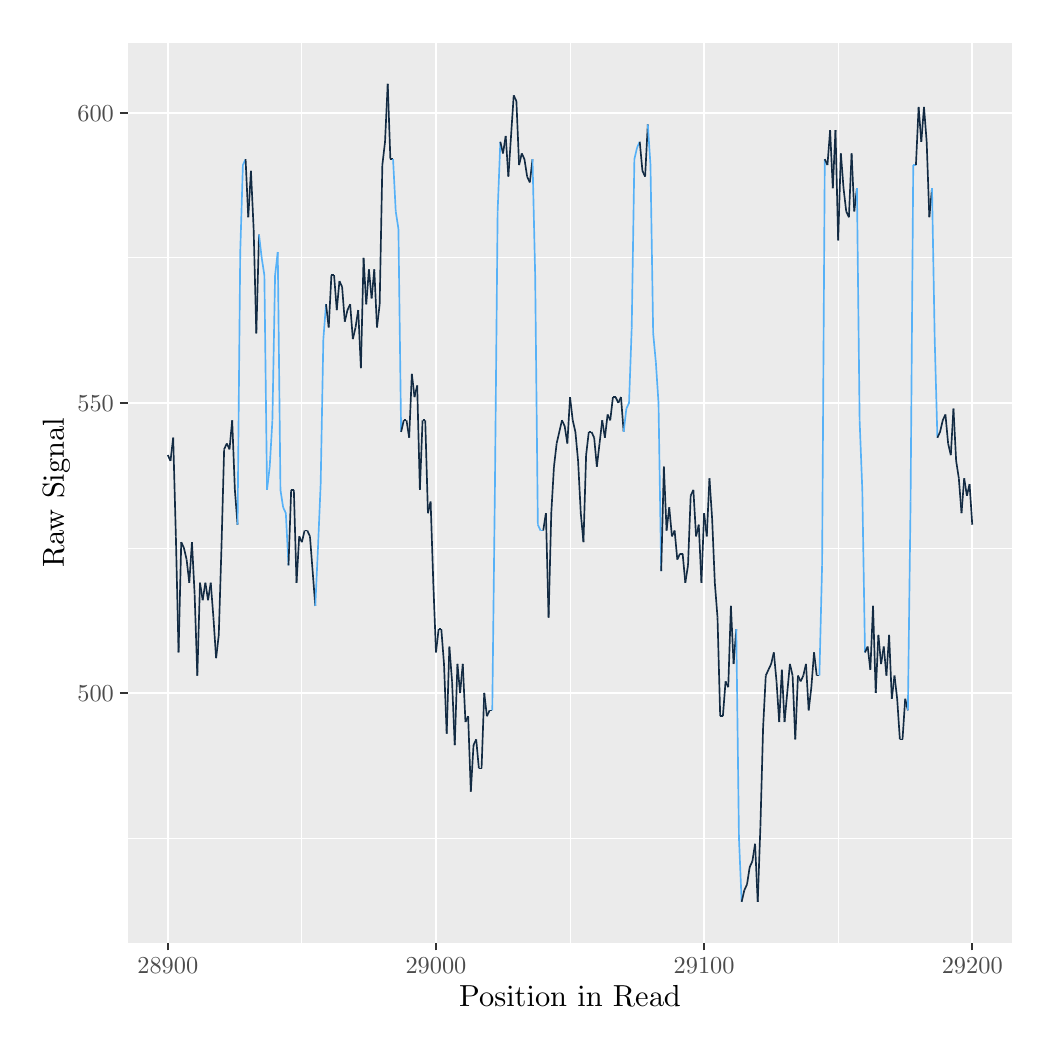
\begin{tikzpicture}[x=1pt,y=1pt]
\definecolor{fillColor}{RGB}{255,255,255}
\path[use as bounding box,fill=fillColor,fill opacity=0.00] (0,0) rectangle (361.35,361.35);
\begin{scope}
\path[clip] (  0.00,  0.00) rectangle (361.35,361.35);
\definecolor{drawColor}{RGB}{255,255,255}
\definecolor{fillColor}{RGB}{255,255,255}

\path[draw=drawColor,line width= 0.6pt,line join=round,line cap=round,fill=fillColor] (  0.00,  0.00) rectangle (361.35,361.35);
\end{scope}
\begin{scope}
\path[clip] ( 36.11, 30.69) rectangle (355.85,355.85);
\definecolor{fillColor}{gray}{0.92}

\path[fill=fillColor] ( 36.11, 30.69) rectangle (355.85,355.85);
\definecolor{drawColor}{RGB}{255,255,255}

\path[draw=drawColor,line width= 0.3pt,line join=round] ( 36.11, 68.53) --
	(355.85, 68.53);

\path[draw=drawColor,line width= 0.3pt,line join=round] ( 36.11,173.35) --
	(355.85,173.35);

\path[draw=drawColor,line width= 0.3pt,line join=round] ( 36.11,278.18) --
	(355.85,278.18);

\path[draw=drawColor,line width= 0.3pt,line join=round] ( 99.09, 30.69) --
	( 99.09,355.85);

\path[draw=drawColor,line width= 0.3pt,line join=round] (195.98, 30.69) --
	(195.98,355.85);

\path[draw=drawColor,line width= 0.3pt,line join=round] (292.87, 30.69) --
	(292.87,355.85);

\path[draw=drawColor,line width= 0.6pt,line join=round] ( 36.11,120.94) --
	(355.85,120.94);

\path[draw=drawColor,line width= 0.6pt,line join=round] ( 36.11,225.76) --
	(355.85,225.76);

\path[draw=drawColor,line width= 0.6pt,line join=round] ( 36.11,330.59) --
	(355.85,330.59);

\path[draw=drawColor,line width= 0.6pt,line join=round] ( 50.64, 30.69) --
	( 50.64,355.85);

\path[draw=drawColor,line width= 0.6pt,line join=round] (147.54, 30.69) --
	(147.54,355.85);

\path[draw=drawColor,line width= 0.6pt,line join=round] (244.43, 30.69) --
	(244.43,355.85);

\path[draw=drawColor,line width= 0.6pt,line join=round] (341.32, 30.69) --
	(341.32,355.85);
\definecolor{drawColor}{RGB}{19,43,67}

\path[draw=drawColor,line width= 0.6pt,line join=round] ( 50.64,206.90) -- ( 51.61,204.80);

\path[draw=drawColor,line width= 0.6pt,line join=round] ( 51.61,204.80) -- ( 52.58,213.18);

\path[draw=drawColor,line width= 0.6pt,line join=round] ( 52.58,213.18) -- ( 53.55,177.54);

\path[draw=drawColor,line width= 0.6pt,line join=round] ( 53.55,177.54) -- ( 54.52,135.61);

\path[draw=drawColor,line width= 0.6pt,line join=round] ( 54.52,135.61) -- ( 55.49,175.45);

\path[draw=drawColor,line width= 0.6pt,line join=round] ( 55.49,175.45) -- ( 56.46,173.35);

\path[draw=drawColor,line width= 0.6pt,line join=round] ( 56.46,173.35) -- ( 57.43,169.16);

\path[draw=drawColor,line width= 0.6pt,line join=round] ( 57.43,169.16) -- ( 58.40,160.77);

\path[draw=drawColor,line width= 0.6pt,line join=round] ( 58.40,160.77) -- ( 59.36,175.45);

\path[draw=drawColor,line width= 0.6pt,line join=round] ( 59.36,175.45) -- ( 60.33,156.58);

\path[draw=drawColor,line width= 0.6pt,line join=round] ( 60.33,156.58) -- ( 61.30,127.23);

\path[draw=drawColor,line width= 0.6pt,line join=round] ( 61.30,127.23) -- ( 62.27,160.77);

\path[draw=drawColor,line width= 0.6pt,line join=round] ( 62.27,160.77) -- ( 63.24,154.48);

\path[draw=drawColor,line width= 0.6pt,line join=round] ( 63.24,154.48) -- ( 64.21,160.77);

\path[draw=drawColor,line width= 0.6pt,line join=round] ( 64.21,160.77) -- ( 65.18,154.48);

\path[draw=drawColor,line width= 0.6pt,line join=round] ( 65.18,154.48) -- ( 66.15,160.77);

\path[draw=drawColor,line width= 0.6pt,line join=round] ( 66.15,160.77) -- ( 67.12,148.19);

\path[draw=drawColor,line width= 0.6pt,line join=round] ( 67.12,148.19) -- ( 68.09,133.52);

\path[draw=drawColor,line width= 0.6pt,line join=round] ( 68.09,133.52) -- ( 69.05,141.90);

\path[draw=drawColor,line width= 0.6pt,line join=round] ( 69.05,141.90) -- ( 70.02,173.35);

\path[draw=drawColor,line width= 0.6pt,line join=round] ( 70.02,173.35) -- ( 70.99,208.99);

\path[draw=drawColor,line width= 0.6pt,line join=round] ( 70.99,208.99) -- ( 71.96,211.09);

\path[draw=drawColor,line width= 0.6pt,line join=round] ( 71.96,211.09) -- ( 72.93,208.99);

\path[draw=drawColor,line width= 0.6pt,line join=round] ( 72.93,208.99) -- ( 73.90,219.47);

\path[draw=drawColor,line width= 0.6pt,line join=round] ( 73.90,219.47) -- ( 74.87,194.32);

\path[draw=drawColor,line width= 0.6pt,line join=round] ( 74.87,194.32) -- ( 75.84,181.74);
\definecolor{drawColor}{RGB}{86,177,247}

\path[draw=drawColor,line width= 0.6pt,line join=round] ( 75.84,181.74) -- ( 76.81,280.27);

\path[draw=drawColor,line width= 0.6pt,line join=round] ( 76.81,280.27) -- ( 77.77,311.72);

\path[draw=drawColor,line width= 0.6pt,line join=round] ( 77.77,311.72) -- ( 78.74,313.82);
\definecolor{drawColor}{RGB}{19,43,67}

\path[draw=drawColor,line width= 0.6pt,line join=round] ( 78.74,313.82) -- ( 79.71,292.85);

\path[draw=drawColor,line width= 0.6pt,line join=round] ( 79.71,292.85) -- ( 80.68,309.62);

\path[draw=drawColor,line width= 0.6pt,line join=round] ( 80.68,309.62) -- ( 81.65,288.66);

\path[draw=drawColor,line width= 0.6pt,line join=round] ( 81.65,288.66) -- ( 82.62,250.92);

\path[draw=drawColor,line width= 0.6pt,line join=round] ( 82.62,250.92) -- ( 83.59,286.56);
\definecolor{drawColor}{RGB}{86,177,247}

\path[draw=drawColor,line width= 0.6pt,line join=round] ( 83.59,286.56) -- ( 84.56,278.18);

\path[draw=drawColor,line width= 0.6pt,line join=round] ( 84.56,278.18) -- ( 85.53,271.89);

\path[draw=drawColor,line width= 0.6pt,line join=round] ( 85.53,271.89) -- ( 86.49,194.32);

\path[draw=drawColor,line width= 0.6pt,line join=round] ( 86.49,194.32) -- ( 87.46,202.70);

\path[draw=drawColor,line width= 0.6pt,line join=round] ( 87.46,202.70) -- ( 88.43,219.47);

\path[draw=drawColor,line width= 0.6pt,line join=round] ( 88.43,219.47) -- ( 89.40,271.89);

\path[draw=drawColor,line width= 0.6pt,line join=round] ( 89.40,271.89) -- ( 90.37,280.27);

\path[draw=drawColor,line width= 0.6pt,line join=round] ( 90.37,280.27) -- ( 91.34,194.32);

\path[draw=drawColor,line width= 0.6pt,line join=round] ( 91.34,194.32) -- ( 92.31,188.03);

\path[draw=drawColor,line width= 0.6pt,line join=round] ( 92.31,188.03) -- ( 93.28,185.93);

\path[draw=drawColor,line width= 0.6pt,line join=round] ( 93.28,185.93) -- ( 94.25,167.06);
\definecolor{drawColor}{RGB}{19,43,67}

\path[draw=drawColor,line width= 0.6pt,line join=round] ( 94.25,167.06) -- ( 95.21,194.32);

\path[draw=drawColor,line width= 0.6pt,line join=round] ( 95.21,194.32) -- ( 96.18,194.32);

\path[draw=drawColor,line width= 0.6pt,line join=round] ( 96.18,194.32) -- ( 97.15,160.77);

\path[draw=drawColor,line width= 0.6pt,line join=round] ( 97.15,160.77) -- ( 98.12,177.54);

\path[draw=drawColor,line width= 0.6pt,line join=round] ( 98.12,177.54) -- ( 99.09,175.45);

\path[draw=drawColor,line width= 0.6pt,line join=round] ( 99.09,175.45) -- (100.06,179.64);

\path[draw=drawColor,line width= 0.6pt,line join=round] (100.06,179.64) -- (101.03,179.64);

\path[draw=drawColor,line width= 0.6pt,line join=round] (101.03,179.64) -- (102.00,177.54);

\path[draw=drawColor,line width= 0.6pt,line join=round] (102.00,177.54) -- (102.97,164.97);

\path[draw=drawColor,line width= 0.6pt,line join=round] (102.97,164.97) -- (103.93,152.39);
\definecolor{drawColor}{RGB}{86,177,247}

\path[draw=drawColor,line width= 0.6pt,line join=round] (103.93,152.39) -- (104.90,173.35);

\path[draw=drawColor,line width= 0.6pt,line join=round] (104.90,173.35) -- (105.87,196.41);

\path[draw=drawColor,line width= 0.6pt,line join=round] (105.87,196.41) -- (106.84,248.82);

\path[draw=drawColor,line width= 0.6pt,line join=round] (106.84,248.82) -- (107.81,261.40);
\definecolor{drawColor}{RGB}{19,43,67}

\path[draw=drawColor,line width= 0.6pt,line join=round] (107.81,261.40) -- (108.78,253.02);

\path[draw=drawColor,line width= 0.6pt,line join=round] (108.78,253.02) -- (109.75,271.89);

\path[draw=drawColor,line width= 0.6pt,line join=round] (109.75,271.89) -- (110.72,271.89);

\path[draw=drawColor,line width= 0.6pt,line join=round] (110.72,271.89) -- (111.69,259.31);

\path[draw=drawColor,line width= 0.6pt,line join=round] (111.69,259.31) -- (112.65,269.79);

\path[draw=drawColor,line width= 0.6pt,line join=round] (112.65,269.79) -- (113.62,267.69);

\path[draw=drawColor,line width= 0.6pt,line join=round] (113.62,267.69) -- (114.59,255.11);

\path[draw=drawColor,line width= 0.6pt,line join=round] (114.59,255.11) -- (115.56,259.31);

\path[draw=drawColor,line width= 0.6pt,line join=round] (115.56,259.31) -- (116.53,261.40);

\path[draw=drawColor,line width= 0.6pt,line join=round] (116.53,261.40) -- (117.50,248.82);

\path[draw=drawColor,line width= 0.6pt,line join=round] (117.50,248.82) -- (118.47,253.02);

\path[draw=drawColor,line width= 0.6pt,line join=round] (118.47,253.02) -- (119.44,259.31);

\path[draw=drawColor,line width= 0.6pt,line join=round] (119.44,259.31) -- (120.41,238.34);

\path[draw=drawColor,line width= 0.6pt,line join=round] (120.41,238.34) -- (121.37,278.18);

\path[draw=drawColor,line width= 0.6pt,line join=round] (121.37,278.18) -- (122.34,261.40);

\path[draw=drawColor,line width= 0.6pt,line join=round] (122.34,261.40) -- (123.31,273.98);

\path[draw=drawColor,line width= 0.6pt,line join=round] (123.31,273.98) -- (124.28,263.50);

\path[draw=drawColor,line width= 0.6pt,line join=round] (124.28,263.50) -- (125.25,273.98);

\path[draw=drawColor,line width= 0.6pt,line join=round] (125.25,273.98) -- (126.22,253.02);

\path[draw=drawColor,line width= 0.6pt,line join=round] (126.22,253.02) -- (127.19,261.40);

\path[draw=drawColor,line width= 0.6pt,line join=round] (127.19,261.40) -- (128.16,311.72);

\path[draw=drawColor,line width= 0.6pt,line join=round] (128.16,311.72) -- (129.13,320.11);

\path[draw=drawColor,line width= 0.6pt,line join=round] (129.13,320.11) -- (130.10,341.07);

\path[draw=drawColor,line width= 0.6pt,line join=round] (130.10,341.07) -- (131.06,313.82);

\path[draw=drawColor,line width= 0.6pt,line join=round] (131.06,313.82) -- (132.03,313.82);
\definecolor{drawColor}{RGB}{86,177,247}

\path[draw=drawColor,line width= 0.6pt,line join=round] (132.03,313.82) -- (133.00,294.95);

\path[draw=drawColor,line width= 0.6pt,line join=round] (133.00,294.95) -- (133.97,288.66);

\path[draw=drawColor,line width= 0.6pt,line join=round] (133.97,288.66) -- (134.94,215.28);
\definecolor{drawColor}{RGB}{19,43,67}

\path[draw=drawColor,line width= 0.6pt,line join=round] (134.94,215.28) -- (135.91,219.47);

\path[draw=drawColor,line width= 0.6pt,line join=round] (135.91,219.47) -- (136.88,219.47);

\path[draw=drawColor,line width= 0.6pt,line join=round] (136.88,219.47) -- (137.85,213.18);

\path[draw=drawColor,line width= 0.6pt,line join=round] (137.85,213.18) -- (138.82,236.25);

\path[draw=drawColor,line width= 0.6pt,line join=round] (138.82,236.25) -- (139.78,227.86);

\path[draw=drawColor,line width= 0.6pt,line join=round] (139.78,227.86) -- (140.75,232.05);

\path[draw=drawColor,line width= 0.6pt,line join=round] (140.75,232.05) -- (141.72,194.32);

\path[draw=drawColor,line width= 0.6pt,line join=round] (141.72,194.32) -- (142.69,219.47);

\path[draw=drawColor,line width= 0.6pt,line join=round] (142.69,219.47) -- (143.66,219.47);

\path[draw=drawColor,line width= 0.6pt,line join=round] (143.66,219.47) -- (144.63,185.93);

\path[draw=drawColor,line width= 0.6pt,line join=round] (144.63,185.93) -- (145.60,190.12);

\path[draw=drawColor,line width= 0.6pt,line join=round] (145.60,190.12) -- (146.57,160.77);

\path[draw=drawColor,line width= 0.6pt,line join=round] (146.57,160.77) -- (147.54,135.61);

\path[draw=drawColor,line width= 0.6pt,line join=round] (147.54,135.61) -- (148.50,144.00);

\path[draw=drawColor,line width= 0.6pt,line join=round] (148.50,144.00) -- (149.47,144.00);

\path[draw=drawColor,line width= 0.6pt,line join=round] (149.47,144.00) -- (150.44,131.42);

\path[draw=drawColor,line width= 0.6pt,line join=round] (150.44,131.42) -- (151.41,106.26);

\path[draw=drawColor,line width= 0.6pt,line join=round] (151.41,106.26) -- (152.38,137.71);

\path[draw=drawColor,line width= 0.6pt,line join=round] (152.38,137.71) -- (153.35,125.13);

\path[draw=drawColor,line width= 0.6pt,line join=round] (153.35,125.13) -- (154.32,102.07);

\path[draw=drawColor,line width= 0.6pt,line join=round] (154.32,102.07) -- (155.29,131.42);

\path[draw=drawColor,line width= 0.6pt,line join=round] (155.29,131.42) -- (156.26,120.94);

\path[draw=drawColor,line width= 0.6pt,line join=round] (156.26,120.94) -- (157.22,131.42);

\path[draw=drawColor,line width= 0.6pt,line join=round] (157.22,131.42) -- (158.19,110.46);

\path[draw=drawColor,line width= 0.6pt,line join=round] (158.19,110.46) -- (159.16,112.55);

\path[draw=drawColor,line width= 0.6pt,line join=round] (159.16,112.55) -- (160.13, 85.30);

\path[draw=drawColor,line width= 0.6pt,line join=round] (160.13, 85.30) -- (161.10,102.07);

\path[draw=drawColor,line width= 0.6pt,line join=round] (161.10,102.07) -- (162.07,104.17);

\path[draw=drawColor,line width= 0.6pt,line join=round] (162.07,104.17) -- (163.04, 93.69);

\path[draw=drawColor,line width= 0.6pt,line join=round] (163.04, 93.69) -- (164.01, 93.69);

\path[draw=drawColor,line width= 0.6pt,line join=round] (164.01, 93.69) -- (164.98,120.94);

\path[draw=drawColor,line width= 0.6pt,line join=round] (164.98,120.94) -- (165.94,112.55);

\path[draw=drawColor,line width= 0.6pt,line join=round] (165.94,112.55) -- (166.91,114.65);

\path[draw=drawColor,line width= 0.6pt,line join=round] (166.91,114.65) -- (167.88,114.65);
\definecolor{drawColor}{RGB}{86,177,247}

\path[draw=drawColor,line width= 0.6pt,line join=round] (167.88,114.65) -- (168.85,196.41);

\path[draw=drawColor,line width= 0.6pt,line join=round] (168.85,196.41) -- (169.82,294.95);

\path[draw=drawColor,line width= 0.6pt,line join=round] (169.82,294.95) -- (170.79,320.11);
\definecolor{drawColor}{RGB}{19,43,67}

\path[draw=drawColor,line width= 0.6pt,line join=round] (170.79,320.11) -- (171.76,315.91);

\path[draw=drawColor,line width= 0.6pt,line join=round] (171.76,315.91) -- (172.73,322.20);

\path[draw=drawColor,line width= 0.6pt,line join=round] (172.73,322.20) -- (173.70,307.53);

\path[draw=drawColor,line width= 0.6pt,line join=round] (173.70,307.53) -- (174.66,322.20);

\path[draw=drawColor,line width= 0.6pt,line join=round] (174.66,322.20) -- (175.63,336.88);

\path[draw=drawColor,line width= 0.6pt,line join=round] (175.63,336.88) -- (176.60,334.78);

\path[draw=drawColor,line width= 0.6pt,line join=round] (176.60,334.78) -- (177.57,311.72);

\path[draw=drawColor,line width= 0.6pt,line join=round] (177.57,311.72) -- (178.54,315.91);

\path[draw=drawColor,line width= 0.6pt,line join=round] (178.54,315.91) -- (179.51,313.82);

\path[draw=drawColor,line width= 0.6pt,line join=round] (179.51,313.82) -- (180.48,307.53);

\path[draw=drawColor,line width= 0.6pt,line join=round] (180.48,307.53) -- (181.45,305.43);

\path[draw=drawColor,line width= 0.6pt,line join=round] (181.45,305.43) -- (182.42,313.82);
\definecolor{drawColor}{RGB}{86,177,247}

\path[draw=drawColor,line width= 0.6pt,line join=round] (182.42,313.82) -- (183.38,271.89);

\path[draw=drawColor,line width= 0.6pt,line join=round] (183.38,271.89) -- (184.35,181.74);

\path[draw=drawColor,line width= 0.6pt,line join=round] (184.35,181.74) -- (185.32,179.64);

\path[draw=drawColor,line width= 0.6pt,line join=round] (185.32,179.64) -- (186.29,179.64);
\definecolor{drawColor}{RGB}{19,43,67}

\path[draw=drawColor,line width= 0.6pt,line join=round] (186.29,179.64) -- (187.26,185.93);

\path[draw=drawColor,line width= 0.6pt,line join=round] (187.26,185.93) -- (188.23,148.19);

\path[draw=drawColor,line width= 0.6pt,line join=round] (188.23,148.19) -- (189.20,185.93);

\path[draw=drawColor,line width= 0.6pt,line join=round] (189.20,185.93) -- (190.17,202.70);

\path[draw=drawColor,line width= 0.6pt,line join=round] (190.17,202.70) -- (191.14,211.09);

\path[draw=drawColor,line width= 0.6pt,line join=round] (191.14,211.09) -- (192.10,215.28);

\path[draw=drawColor,line width= 0.6pt,line join=round] (192.10,215.28) -- (193.07,219.47);

\path[draw=drawColor,line width= 0.6pt,line join=round] (193.07,219.47) -- (194.04,217.38);

\path[draw=drawColor,line width= 0.6pt,line join=round] (194.04,217.38) -- (195.01,211.09);

\path[draw=drawColor,line width= 0.6pt,line join=round] (195.01,211.09) -- (195.98,227.86);

\path[draw=drawColor,line width= 0.6pt,line join=round] (195.98,227.86) -- (196.95,219.47);

\path[draw=drawColor,line width= 0.6pt,line join=round] (196.95,219.47) -- (197.92,215.28);

\path[draw=drawColor,line width= 0.6pt,line join=round] (197.92,215.28) -- (198.89,204.80);

\path[draw=drawColor,line width= 0.6pt,line join=round] (198.89,204.80) -- (199.86,185.93);

\path[draw=drawColor,line width= 0.6pt,line join=round] (199.86,185.93) -- (200.83,175.45);

\path[draw=drawColor,line width= 0.6pt,line join=round] (200.83,175.45) -- (201.79,206.90);

\path[draw=drawColor,line width= 0.6pt,line join=round] (201.79,206.90) -- (202.76,215.28);

\path[draw=drawColor,line width= 0.6pt,line join=round] (202.76,215.28) -- (203.73,215.28);

\path[draw=drawColor,line width= 0.6pt,line join=round] (203.73,215.28) -- (204.70,213.18);

\path[draw=drawColor,line width= 0.6pt,line join=round] (204.70,213.18) -- (205.67,202.70);

\path[draw=drawColor,line width= 0.6pt,line join=round] (205.67,202.70) -- (206.64,211.09);

\path[draw=drawColor,line width= 0.6pt,line join=round] (206.64,211.09) -- (207.61,219.47);

\path[draw=drawColor,line width= 0.6pt,line join=round] (207.61,219.47) -- (208.58,213.18);

\path[draw=drawColor,line width= 0.6pt,line join=round] (208.58,213.18) -- (209.55,221.57);

\path[draw=drawColor,line width= 0.6pt,line join=round] (209.55,221.57) -- (210.51,219.47);

\path[draw=drawColor,line width= 0.6pt,line join=round] (210.51,219.47) -- (211.48,227.86);

\path[draw=drawColor,line width= 0.6pt,line join=round] (211.48,227.86) -- (212.45,227.86);

\path[draw=drawColor,line width= 0.6pt,line join=round] (212.45,227.86) -- (213.42,225.76);

\path[draw=drawColor,line width= 0.6pt,line join=round] (213.42,225.76) -- (214.39,227.86);

\path[draw=drawColor,line width= 0.6pt,line join=round] (214.39,227.86) -- (215.36,215.28);
\definecolor{drawColor}{RGB}{86,177,247}

\path[draw=drawColor,line width= 0.6pt,line join=round] (215.36,215.28) -- (216.33,223.67);

\path[draw=drawColor,line width= 0.6pt,line join=round] (216.33,223.67) -- (217.30,225.76);

\path[draw=drawColor,line width= 0.6pt,line join=round] (217.30,225.76) -- (218.27,253.02);

\path[draw=drawColor,line width= 0.6pt,line join=round] (218.27,253.02) -- (219.23,313.82);

\path[draw=drawColor,line width= 0.6pt,line join=round] (219.23,313.82) -- (220.20,318.01);

\path[draw=drawColor,line width= 0.6pt,line join=round] (220.20,318.01) -- (221.17,320.11);
\definecolor{drawColor}{RGB}{19,43,67}

\path[draw=drawColor,line width= 0.6pt,line join=round] (221.17,320.11) -- (222.14,309.62);

\path[draw=drawColor,line width= 0.6pt,line join=round] (222.14,309.62) -- (223.11,307.53);

\path[draw=drawColor,line width= 0.6pt,line join=round] (223.11,307.53) -- (224.08,326.39);
\definecolor{drawColor}{RGB}{86,177,247}

\path[draw=drawColor,line width= 0.6pt,line join=round] (224.08,326.39) -- (225.05,311.72);

\path[draw=drawColor,line width= 0.6pt,line join=round] (225.05,311.72) -- (226.02,250.92);

\path[draw=drawColor,line width= 0.6pt,line join=round] (226.02,250.92) -- (226.99,240.44);

\path[draw=drawColor,line width= 0.6pt,line join=round] (226.99,240.44) -- (227.95,225.76);

\path[draw=drawColor,line width= 0.6pt,line join=round] (227.95,225.76) -- (228.92,164.97);
\definecolor{drawColor}{RGB}{19,43,67}

\path[draw=drawColor,line width= 0.6pt,line join=round] (228.92,164.97) -- (229.89,202.70);

\path[draw=drawColor,line width= 0.6pt,line join=round] (229.89,202.70) -- (230.86,179.64);

\path[draw=drawColor,line width= 0.6pt,line join=round] (230.86,179.64) -- (231.83,188.03);

\path[draw=drawColor,line width= 0.6pt,line join=round] (231.83,188.03) -- (232.80,177.54);

\path[draw=drawColor,line width= 0.6pt,line join=round] (232.80,177.54) -- (233.77,179.64);

\path[draw=drawColor,line width= 0.6pt,line join=round] (233.77,179.64) -- (234.74,169.16);

\path[draw=drawColor,line width= 0.6pt,line join=round] (234.74,169.16) -- (235.71,171.25);

\path[draw=drawColor,line width= 0.6pt,line join=round] (235.71,171.25) -- (236.67,171.25);

\path[draw=drawColor,line width= 0.6pt,line join=round] (236.67,171.25) -- (237.64,160.77);

\path[draw=drawColor,line width= 0.6pt,line join=round] (237.64,160.77) -- (238.61,167.06);

\path[draw=drawColor,line width= 0.6pt,line join=round] (238.61,167.06) -- (239.58,192.22);

\path[draw=drawColor,line width= 0.6pt,line join=round] (239.58,192.22) -- (240.55,194.32);

\path[draw=drawColor,line width= 0.6pt,line join=round] (240.55,194.32) -- (241.52,177.54);

\path[draw=drawColor,line width= 0.6pt,line join=round] (241.52,177.54) -- (242.49,181.74);

\path[draw=drawColor,line width= 0.6pt,line join=round] (242.49,181.74) -- (243.46,160.77);

\path[draw=drawColor,line width= 0.6pt,line join=round] (243.46,160.77) -- (244.43,185.93);

\path[draw=drawColor,line width= 0.6pt,line join=round] (244.43,185.93) -- (245.39,177.54);

\path[draw=drawColor,line width= 0.6pt,line join=round] (245.39,177.54) -- (246.36,198.51);

\path[draw=drawColor,line width= 0.6pt,line join=round] (246.36,198.51) -- (247.33,183.83);

\path[draw=drawColor,line width= 0.6pt,line join=round] (247.33,183.83) -- (248.30,160.77);

\path[draw=drawColor,line width= 0.6pt,line join=round] (248.30,160.77) -- (249.27,148.19);

\path[draw=drawColor,line width= 0.6pt,line join=round] (249.27,148.19) -- (250.24,112.55);

\path[draw=drawColor,line width= 0.6pt,line join=round] (250.24,112.55) -- (251.21,112.55);

\path[draw=drawColor,line width= 0.6pt,line join=round] (251.21,112.55) -- (252.18,125.13);

\path[draw=drawColor,line width= 0.6pt,line join=round] (252.18,125.13) -- (253.15,123.04);

\path[draw=drawColor,line width= 0.6pt,line join=round] (253.15,123.04) -- (254.11,152.39);

\path[draw=drawColor,line width= 0.6pt,line join=round] (254.11,152.39) -- (255.08,131.42);

\path[draw=drawColor,line width= 0.6pt,line join=round] (255.08,131.42) -- (256.05,144.00);
\definecolor{drawColor}{RGB}{86,177,247}

\path[draw=drawColor,line width= 0.6pt,line join=round] (256.05,144.00) -- (257.02, 68.53);

\path[draw=drawColor,line width= 0.6pt,line join=round] (257.02, 68.53) -- (257.99, 45.47);
\definecolor{drawColor}{RGB}{19,43,67}

\path[draw=drawColor,line width= 0.6pt,line join=round] (257.99, 45.47) -- (258.96, 49.66);

\path[draw=drawColor,line width= 0.6pt,line join=round] (258.96, 49.66) -- (259.93, 51.76);

\path[draw=drawColor,line width= 0.6pt,line join=round] (259.93, 51.76) -- (260.90, 58.04);

\path[draw=drawColor,line width= 0.6pt,line join=round] (260.90, 58.04) -- (261.87, 60.14);

\path[draw=drawColor,line width= 0.6pt,line join=round] (261.87, 60.14) -- (262.84, 66.43);

\path[draw=drawColor,line width= 0.6pt,line join=round] (262.84, 66.43) -- (263.80, 45.47);

\path[draw=drawColor,line width= 0.6pt,line join=round] (263.80, 45.47) -- (264.77, 72.72);

\path[draw=drawColor,line width= 0.6pt,line join=round] (264.77, 72.72) -- (265.74,108.36);

\path[draw=drawColor,line width= 0.6pt,line join=round] (265.74,108.36) -- (266.71,127.23);

\path[draw=drawColor,line width= 0.6pt,line join=round] (266.71,127.23) -- (267.68,129.33);

\path[draw=drawColor,line width= 0.6pt,line join=round] (267.68,129.33) -- (268.65,131.42);

\path[draw=drawColor,line width= 0.6pt,line join=round] (268.65,131.42) -- (269.62,135.61);

\path[draw=drawColor,line width= 0.6pt,line join=round] (269.62,135.61) -- (270.59,125.13);

\path[draw=drawColor,line width= 0.6pt,line join=round] (270.59,125.13) -- (271.56,110.46);

\path[draw=drawColor,line width= 0.6pt,line join=round] (271.56,110.46) -- (272.52,129.33);

\path[draw=drawColor,line width= 0.6pt,line join=round] (272.52,129.33) -- (273.49,110.46);

\path[draw=drawColor,line width= 0.6pt,line join=round] (273.49,110.46) -- (274.46,120.94);

\path[draw=drawColor,line width= 0.6pt,line join=round] (274.46,120.94) -- (275.43,131.42);

\path[draw=drawColor,line width= 0.6pt,line join=round] (275.43,131.42) -- (276.40,127.23);

\path[draw=drawColor,line width= 0.6pt,line join=round] (276.40,127.23) -- (277.37,104.17);

\path[draw=drawColor,line width= 0.6pt,line join=round] (277.37,104.17) -- (278.34,127.23);

\path[draw=drawColor,line width= 0.6pt,line join=round] (278.34,127.23) -- (279.31,125.13);

\path[draw=drawColor,line width= 0.6pt,line join=round] (279.31,125.13) -- (280.28,127.23);

\path[draw=drawColor,line width= 0.6pt,line join=round] (280.28,127.23) -- (281.24,131.42);

\path[draw=drawColor,line width= 0.6pt,line join=round] (281.24,131.42) -- (282.21,114.65);

\path[draw=drawColor,line width= 0.6pt,line join=round] (282.21,114.65) -- (283.18,123.04);

\path[draw=drawColor,line width= 0.6pt,line join=round] (283.18,123.04) -- (284.15,135.61);

\path[draw=drawColor,line width= 0.6pt,line join=round] (284.15,135.61) -- (285.12,127.23);

\path[draw=drawColor,line width= 0.6pt,line join=round] (285.12,127.23) -- (286.09,127.23);
\definecolor{drawColor}{RGB}{86,177,247}

\path[draw=drawColor,line width= 0.6pt,line join=round] (286.09,127.23) -- (287.06,167.06);

\path[draw=drawColor,line width= 0.6pt,line join=round] (287.06,167.06) -- (288.03,313.82);
\definecolor{drawColor}{RGB}{19,43,67}

\path[draw=drawColor,line width= 0.6pt,line join=round] (288.03,313.82) -- (289.00,311.72);

\path[draw=drawColor,line width= 0.6pt,line join=round] (289.00,311.72) -- (289.96,324.30);

\path[draw=drawColor,line width= 0.6pt,line join=round] (289.96,324.30) -- (290.93,303.33);

\path[draw=drawColor,line width= 0.6pt,line join=round] (290.93,303.33) -- (291.90,324.30);

\path[draw=drawColor,line width= 0.6pt,line join=round] (291.90,324.30) -- (292.87,284.46);

\path[draw=drawColor,line width= 0.6pt,line join=round] (292.87,284.46) -- (293.84,315.91);

\path[draw=drawColor,line width= 0.6pt,line join=round] (293.84,315.91) -- (294.81,303.33);

\path[draw=drawColor,line width= 0.6pt,line join=round] (294.81,303.33) -- (295.78,294.95);

\path[draw=drawColor,line width= 0.6pt,line join=round] (295.78,294.95) -- (296.75,292.85);

\path[draw=drawColor,line width= 0.6pt,line join=round] (296.75,292.85) -- (297.72,315.91);

\path[draw=drawColor,line width= 0.6pt,line join=round] (297.72,315.91) -- (298.68,294.95);

\path[draw=drawColor,line width= 0.6pt,line join=round] (298.68,294.95) -- (299.65,303.33);
\definecolor{drawColor}{RGB}{86,177,247}

\path[draw=drawColor,line width= 0.6pt,line join=round] (299.65,303.33) -- (300.62,219.47);

\path[draw=drawColor,line width= 0.6pt,line join=round] (300.62,219.47) -- (301.59,194.32);

\path[draw=drawColor,line width= 0.6pt,line join=round] (301.59,194.32) -- (302.56,135.61);
\definecolor{drawColor}{RGB}{19,43,67}

\path[draw=drawColor,line width= 0.6pt,line join=round] (302.56,135.61) -- (303.53,137.71);

\path[draw=drawColor,line width= 0.6pt,line join=round] (303.53,137.71) -- (304.50,129.33);

\path[draw=drawColor,line width= 0.6pt,line join=round] (304.50,129.33) -- (305.47,152.39);

\path[draw=drawColor,line width= 0.6pt,line join=round] (305.47,152.39) -- (306.44,120.94);

\path[draw=drawColor,line width= 0.6pt,line join=round] (306.44,120.94) -- (307.40,141.90);

\path[draw=drawColor,line width= 0.6pt,line join=round] (307.40,141.90) -- (308.37,131.42);

\path[draw=drawColor,line width= 0.6pt,line join=round] (308.37,131.42) -- (309.34,137.71);

\path[draw=drawColor,line width= 0.6pt,line join=round] (309.34,137.71) -- (310.31,127.23);

\path[draw=drawColor,line width= 0.6pt,line join=round] (310.31,127.23) -- (311.28,141.90);

\path[draw=drawColor,line width= 0.6pt,line join=round] (311.28,141.90) -- (312.25,118.84);

\path[draw=drawColor,line width= 0.6pt,line join=round] (312.25,118.84) -- (313.22,127.23);

\path[draw=drawColor,line width= 0.6pt,line join=round] (313.22,127.23) -- (314.19,118.84);

\path[draw=drawColor,line width= 0.6pt,line join=round] (314.19,118.84) -- (315.16,104.17);

\path[draw=drawColor,line width= 0.6pt,line join=round] (315.16,104.17) -- (316.12,104.17);

\path[draw=drawColor,line width= 0.6pt,line join=round] (316.12,104.17) -- (317.09,118.84);

\path[draw=drawColor,line width= 0.6pt,line join=round] (317.09,118.84) -- (318.06,114.65);
\definecolor{drawColor}{RGB}{86,177,247}

\path[draw=drawColor,line width= 0.6pt,line join=round] (318.06,114.65) -- (319.03,190.12);

\path[draw=drawColor,line width= 0.6pt,line join=round] (319.03,190.12) -- (320.00,311.72);

\path[draw=drawColor,line width= 0.6pt,line join=round] (320.00,311.72) -- (320.97,311.72);
\definecolor{drawColor}{RGB}{19,43,67}

\path[draw=drawColor,line width= 0.6pt,line join=round] (320.97,311.72) -- (321.94,332.68);

\path[draw=drawColor,line width= 0.6pt,line join=round] (321.94,332.68) -- (322.91,320.11);

\path[draw=drawColor,line width= 0.6pt,line join=round] (322.91,320.11) -- (323.88,332.68);

\path[draw=drawColor,line width= 0.6pt,line join=round] (323.88,332.68) -- (324.85,320.11);

\path[draw=drawColor,line width= 0.6pt,line join=round] (324.85,320.11) -- (325.81,292.85);

\path[draw=drawColor,line width= 0.6pt,line join=round] (325.81,292.85) -- (326.78,303.33);
\definecolor{drawColor}{RGB}{86,177,247}

\path[draw=drawColor,line width= 0.6pt,line join=round] (326.78,303.33) -- (327.75,248.82);

\path[draw=drawColor,line width= 0.6pt,line join=round] (327.75,248.82) -- (328.72,213.18);
\definecolor{drawColor}{RGB}{19,43,67}

\path[draw=drawColor,line width= 0.6pt,line join=round] (328.72,213.18) -- (329.69,215.28);

\path[draw=drawColor,line width= 0.6pt,line join=round] (329.69,215.28) -- (330.66,219.47);

\path[draw=drawColor,line width= 0.6pt,line join=round] (330.66,219.47) -- (331.63,221.57);

\path[draw=drawColor,line width= 0.6pt,line join=round] (331.63,221.57) -- (332.60,211.09);

\path[draw=drawColor,line width= 0.6pt,line join=round] (332.60,211.09) -- (333.57,206.90);

\path[draw=drawColor,line width= 0.6pt,line join=round] (333.57,206.90) -- (334.53,223.67);

\path[draw=drawColor,line width= 0.6pt,line join=round] (334.53,223.67) -- (335.50,204.80);

\path[draw=drawColor,line width= 0.6pt,line join=round] (335.50,204.80) -- (336.47,198.51);

\path[draw=drawColor,line width= 0.6pt,line join=round] (336.47,198.51) -- (337.44,185.93);

\path[draw=drawColor,line width= 0.6pt,line join=round] (337.44,185.93) -- (338.41,198.51);

\path[draw=drawColor,line width= 0.6pt,line join=round] (338.41,198.51) -- (339.38,192.22);

\path[draw=drawColor,line width= 0.6pt,line join=round] (339.38,192.22) -- (340.35,196.41);

\path[draw=drawColor,line width= 0.6pt,line join=round] (340.35,196.41) -- (341.32,181.74);
\end{scope}
\begin{scope}
\path[clip] (  0.00,  0.00) rectangle (361.35,361.35);
\definecolor{drawColor}{gray}{0.30}

\node[text=drawColor,anchor=base east,inner sep=0pt, outer sep=0pt, scale=  0.88] at ( 31.16,117.91) {500};

\node[text=drawColor,anchor=base east,inner sep=0pt, outer sep=0pt, scale=  0.88] at ( 31.16,222.73) {550};

\node[text=drawColor,anchor=base east,inner sep=0pt, outer sep=0pt, scale=  0.88] at ( 31.16,327.56) {600};
\end{scope}
\begin{scope}
\path[clip] (  0.00,  0.00) rectangle (361.35,361.35);
\definecolor{drawColor}{gray}{0.20}

\path[draw=drawColor,line width= 0.6pt,line join=round] ( 33.36,120.94) --
	( 36.11,120.94);

\path[draw=drawColor,line width= 0.6pt,line join=round] ( 33.36,225.76) --
	( 36.11,225.76);

\path[draw=drawColor,line width= 0.6pt,line join=round] ( 33.36,330.59) --
	( 36.11,330.59);
\end{scope}
\begin{scope}
\path[clip] (  0.00,  0.00) rectangle (361.35,361.35);
\definecolor{drawColor}{gray}{0.20}

\path[draw=drawColor,line width= 0.6pt,line join=round] ( 50.64, 27.94) --
	( 50.64, 30.69);

\path[draw=drawColor,line width= 0.6pt,line join=round] (147.54, 27.94) --
	(147.54, 30.69);

\path[draw=drawColor,line width= 0.6pt,line join=round] (244.43, 27.94) --
	(244.43, 30.69);

\path[draw=drawColor,line width= 0.6pt,line join=round] (341.32, 27.94) --
	(341.32, 30.69);
\end{scope}
\begin{scope}
\path[clip] (  0.00,  0.00) rectangle (361.35,361.35);
\definecolor{drawColor}{gray}{0.30}

\node[text=drawColor,anchor=base,inner sep=0pt, outer sep=0pt, scale=  0.88] at ( 50.64, 19.68) {28900};

\node[text=drawColor,anchor=base,inner sep=0pt, outer sep=0pt, scale=  0.88] at (147.54, 19.68) {29000};

\node[text=drawColor,anchor=base,inner sep=0pt, outer sep=0pt, scale=  0.88] at (244.43, 19.68) {29100};

\node[text=drawColor,anchor=base,inner sep=0pt, outer sep=0pt, scale=  0.88] at (341.32, 19.68) {29200};
\end{scope}
\begin{scope}
\path[clip] (  0.00,  0.00) rectangle (361.35,361.35);
\definecolor{drawColor}{RGB}{0,0,0}

\node[text=drawColor,anchor=base,inner sep=0pt, outer sep=0pt, scale=  1.10] at (195.98,  7.64) {Position in Read};
\end{scope}
\begin{scope}
\path[clip] (  0.00,  0.00) rectangle (361.35,361.35);
\definecolor{drawColor}{RGB}{0,0,0}

\node[text=drawColor,rotate= 90.00,anchor=base,inner sep=0pt, outer sep=0pt, scale=  1.10] at ( 13.08,193.27) {Raw Signal};
\end{scope}
\end{tikzpicture}
